\chapter{場景建立}
\section{匯入球場及球員}
File-Import-Mesh,選擇要匯入的檔案匯入球場,如(圖.\ref{匯入球場stl檔}) 。\\
\begin{figure}[hbt!]
\begin{center}
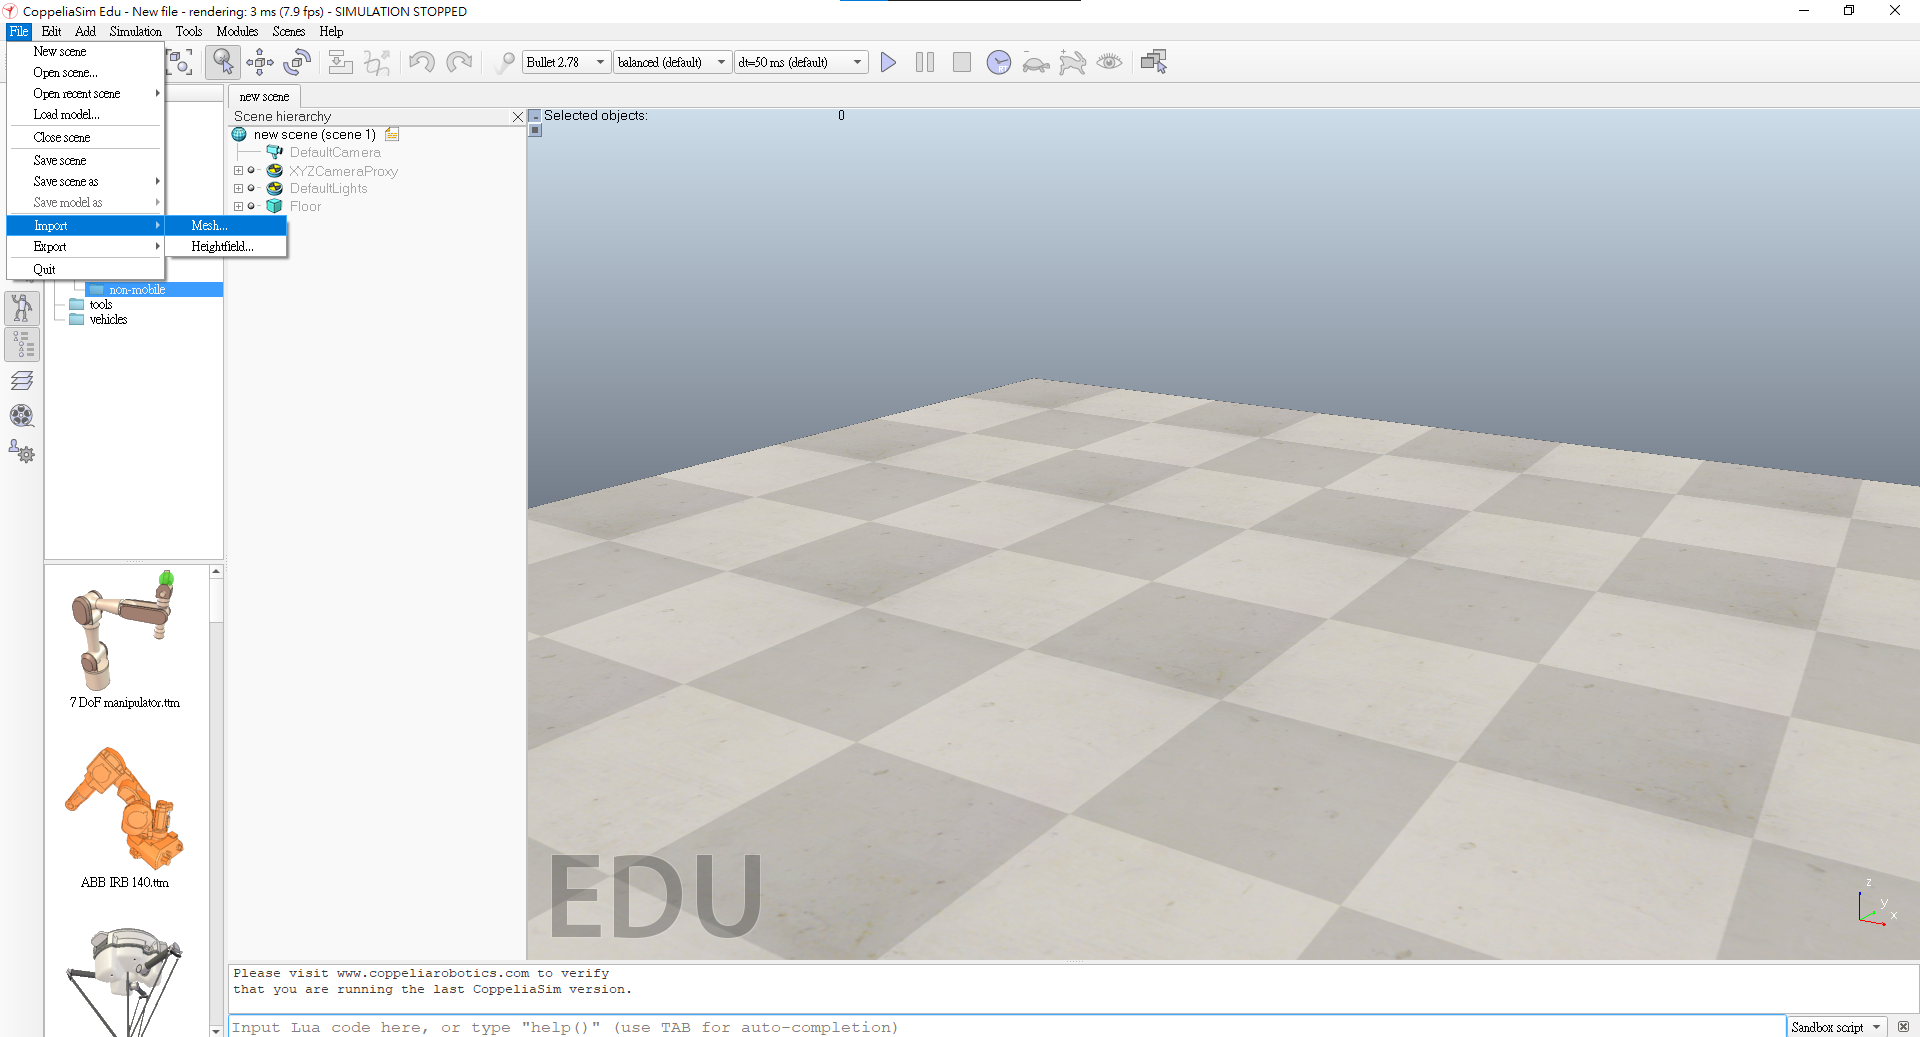
\includegraphics[width=12cm]{匯入球場1}
\caption{\Large 匯入球場stl檔}\label{匯入球場stl檔}
\end{center}
\end{figure} 
\begin{figure}[hbt!]
\begin{center}
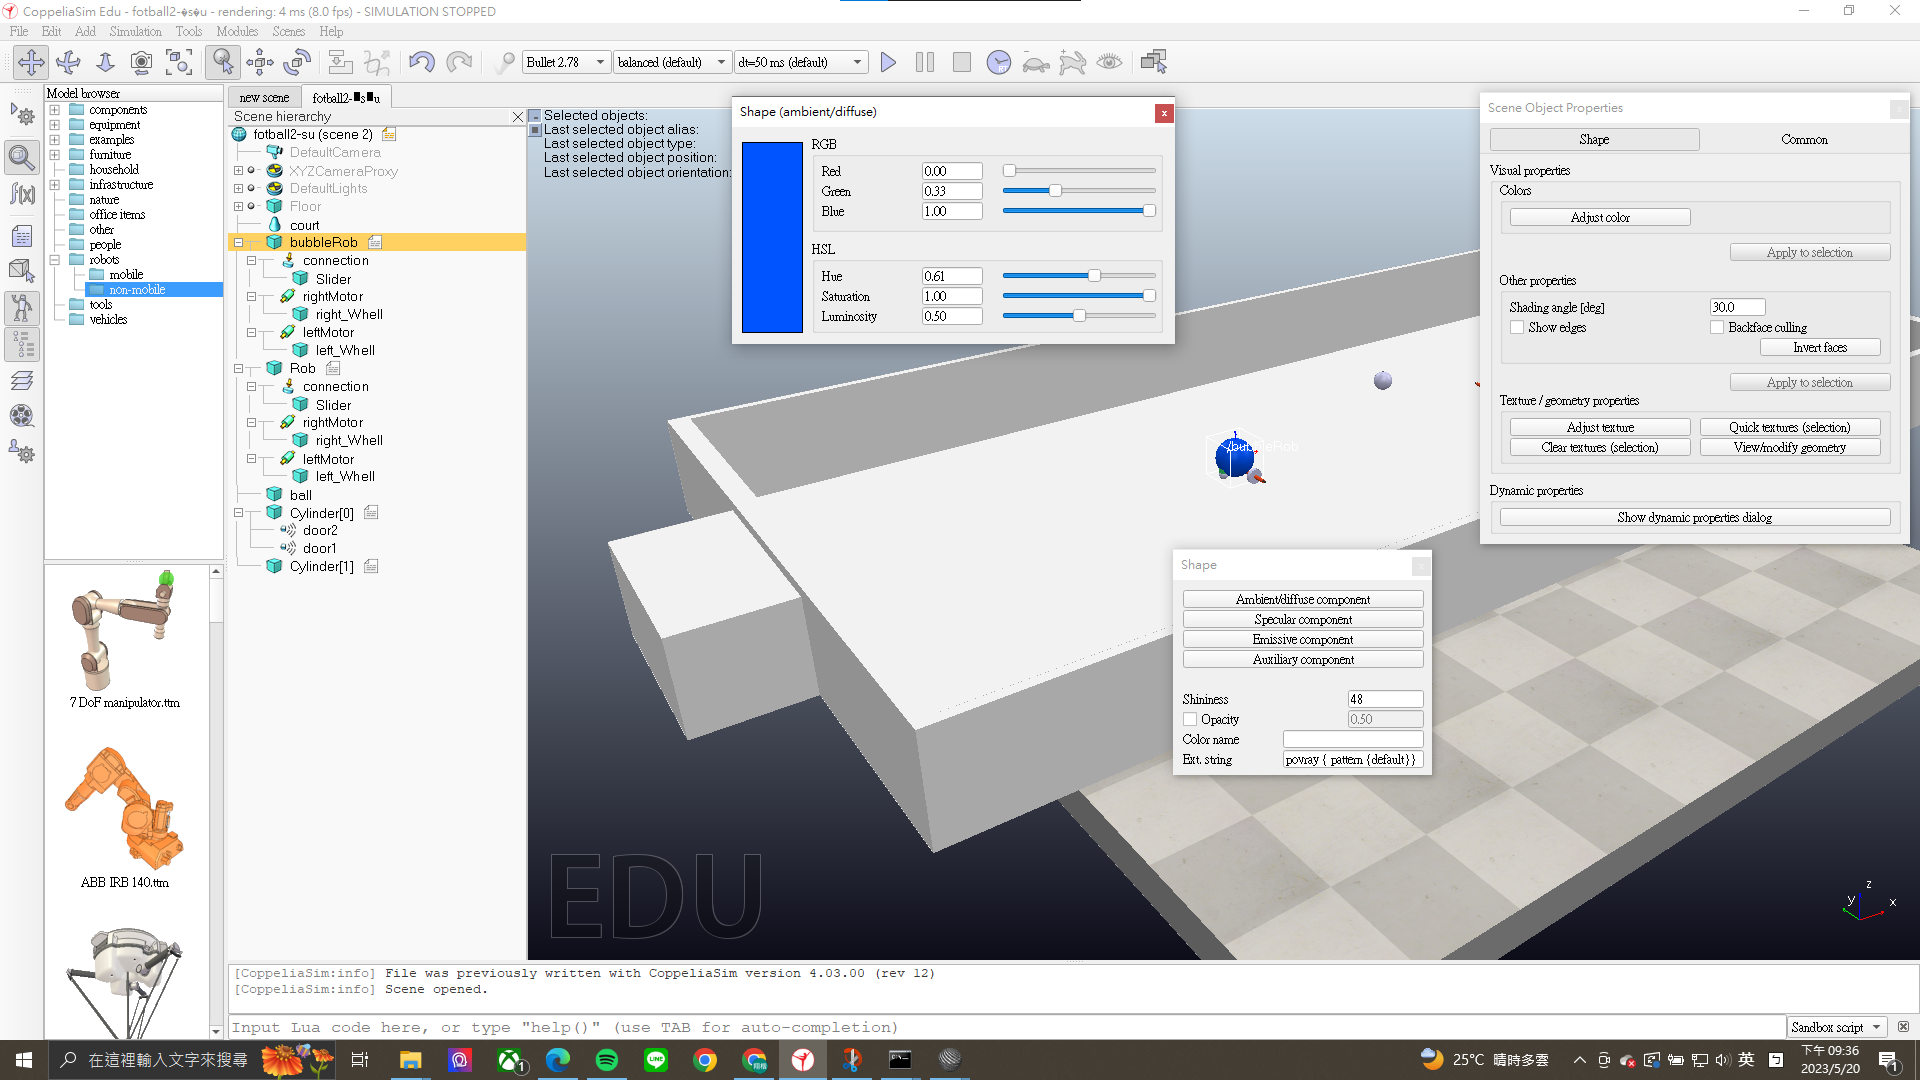
\includegraphics[width=12cm]{變色}
\caption{\Large 改變球員顏色}\label{改變球員顏色}
\end{center}
\end{figure} 
接著依序匯入球員及球,並且作球員顏色的更動,如(圖.\ref{改變球員顏色})。\\
變色方法:點選本體旁邊圖示-Adjust color-Amibient/diffuse component-拉動RGB調整顏色即可。\\
\newpage
\section{記分板建立}
建立第一版記分板做為測試用途。\\
\begin{figure}[hbt!]
\begin{center}
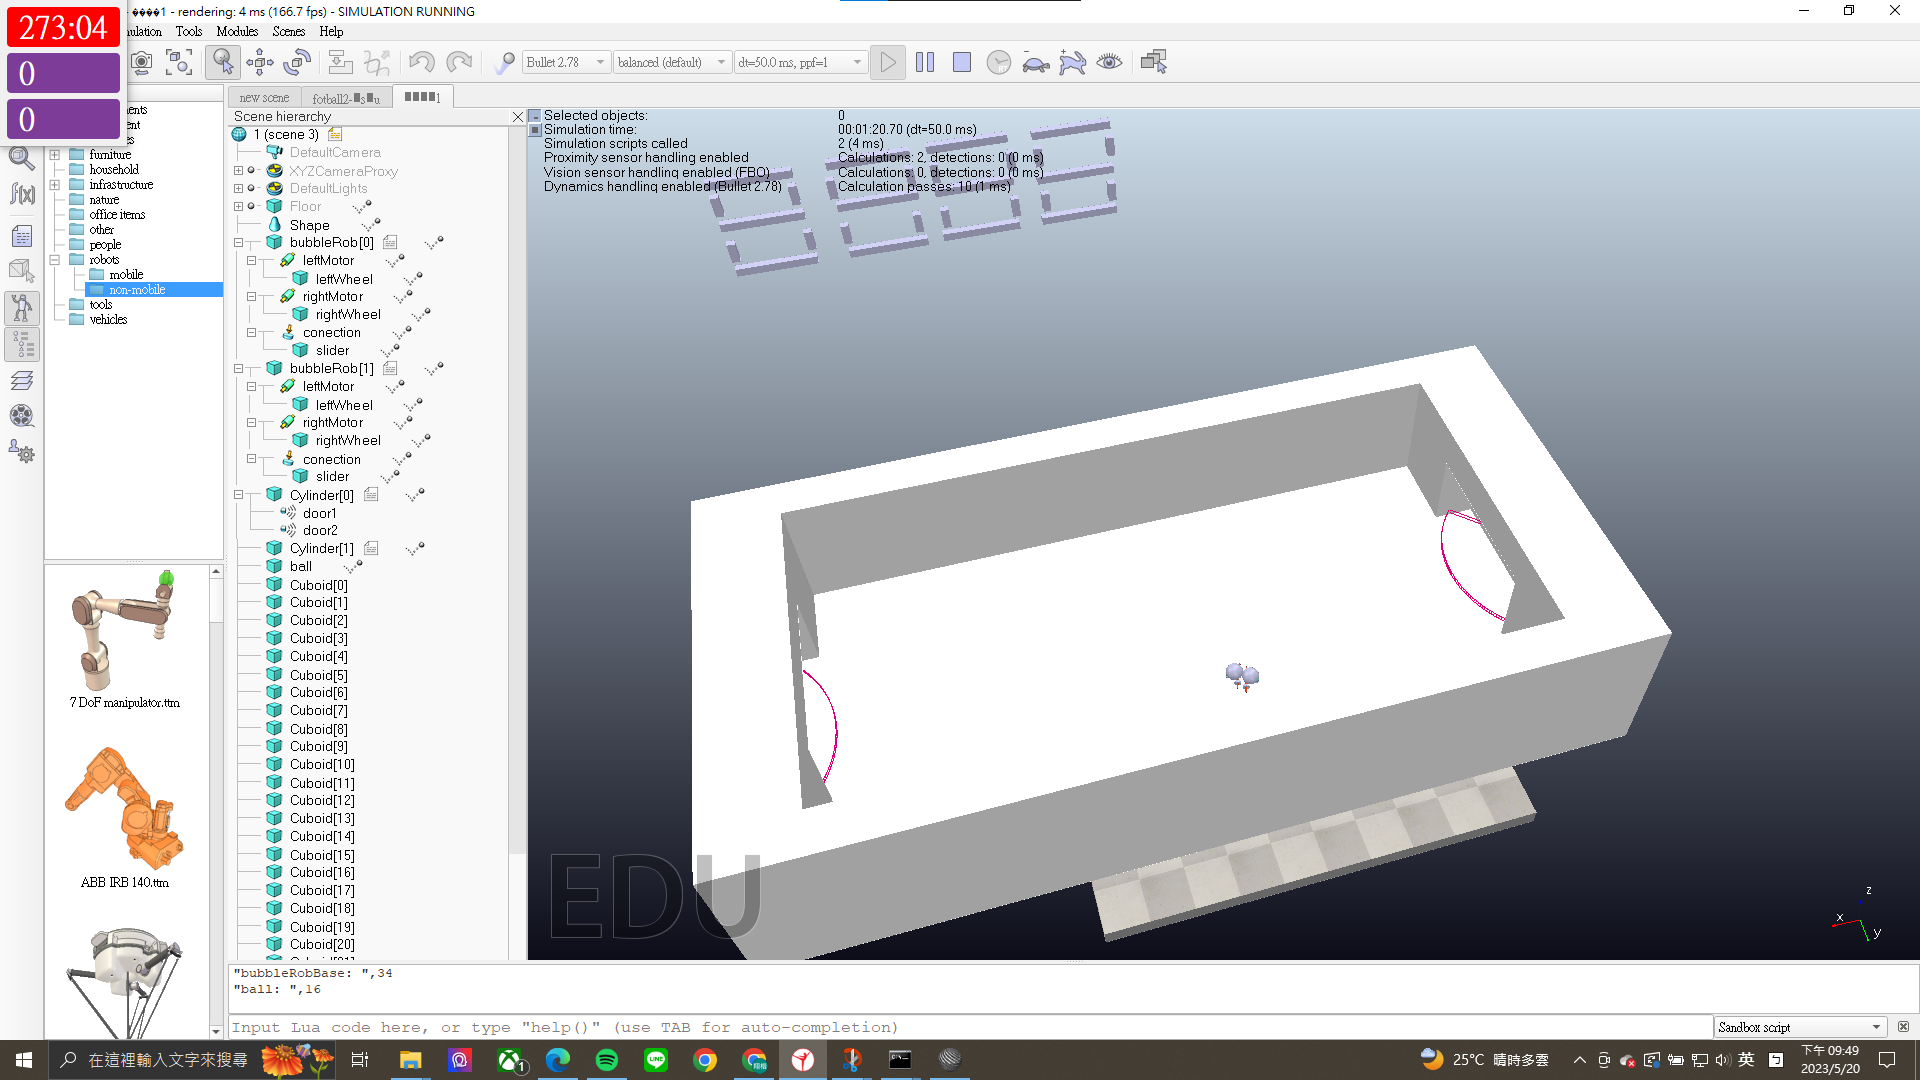
\includegraphics[width=12cm]{測試}
\caption{\Large 測試用記分板}\label{測試用記分板}
\end{center}
\end{figure} \\
接著我們使用Onshape繪製了第二版記分板,匯入後進行爆炸拆件;步驟為Edit-Gourping-Divide selected shape。因為我們是使用變換物件顏色來顯示得分數字,所以物件導入後的拆件動作件特別重要。\\
但由於第二版記分板,無法在Coppeliasim爆炸成個別零件,無法達成我們想改變計分板顏色來實現計分功能的計畫,因此沒有採用。
\begin{figure}[hbt!]
\begin{center}
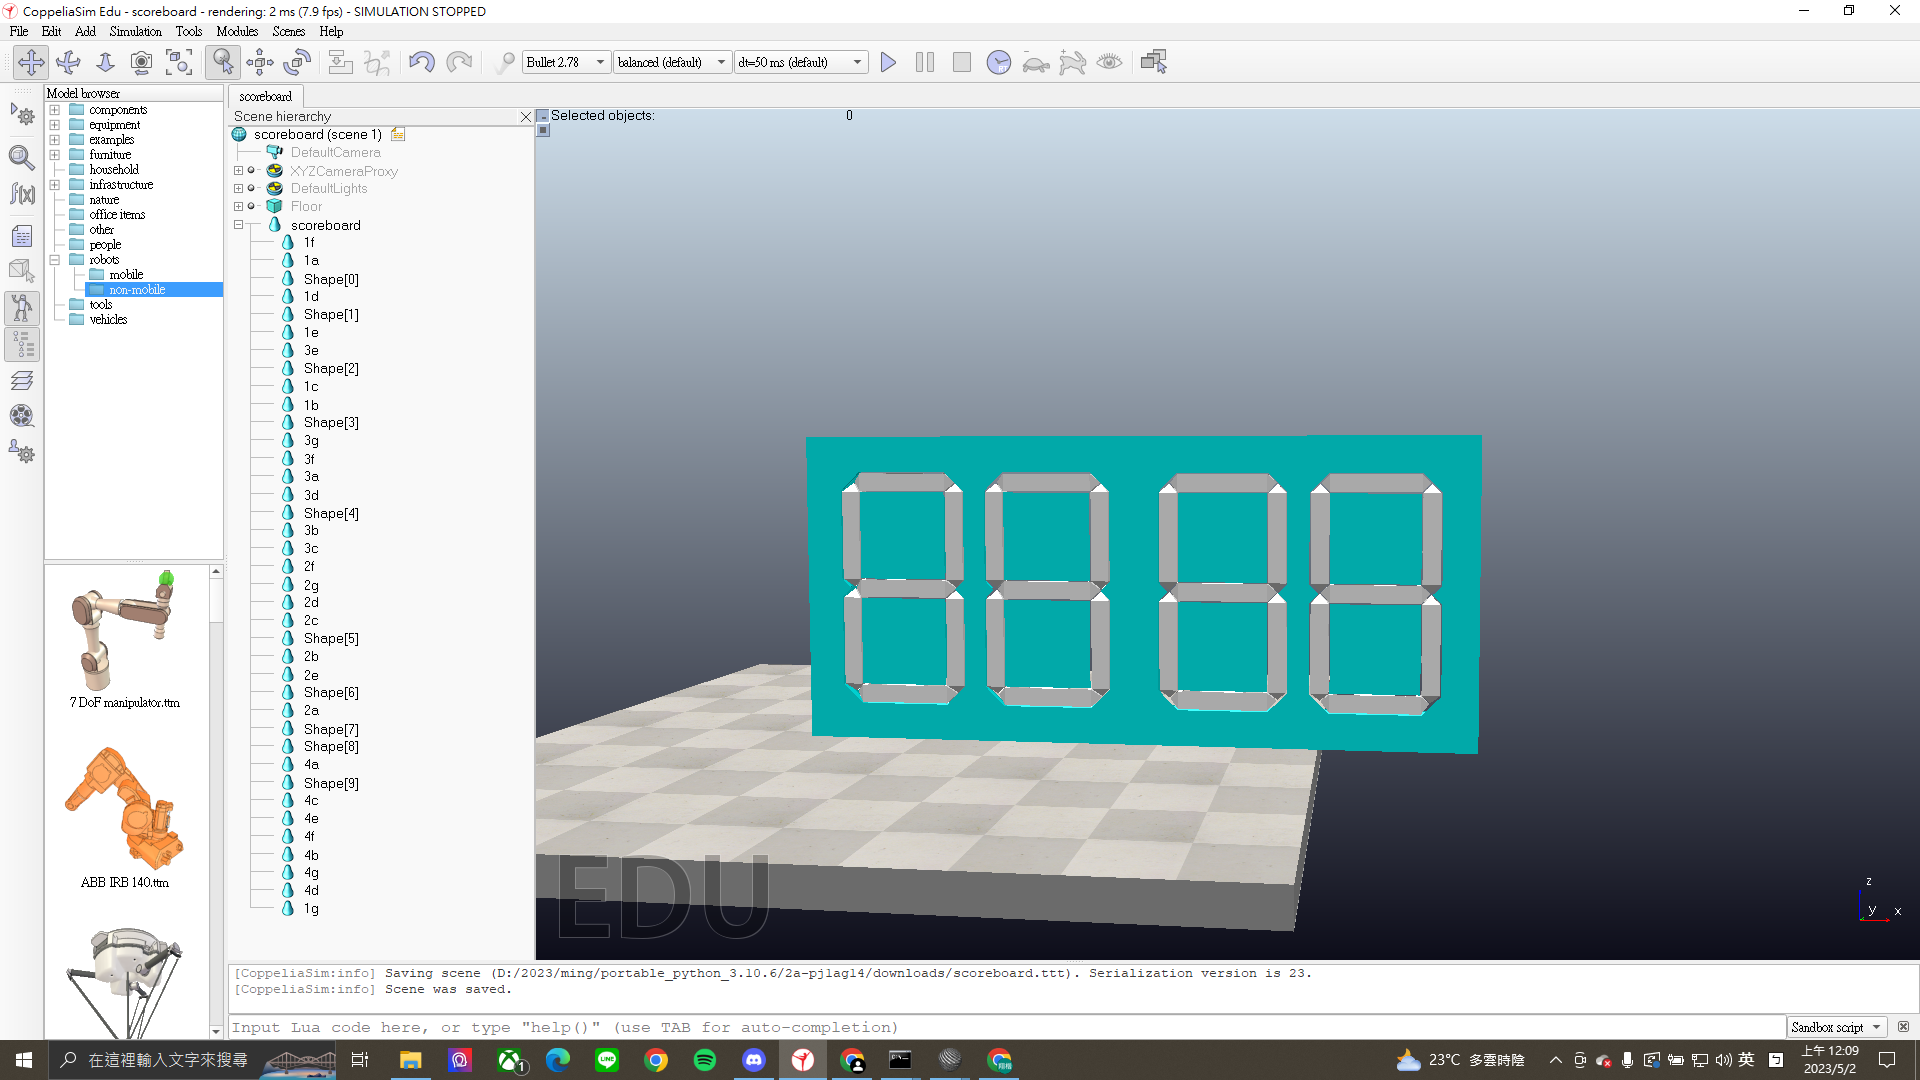
\includegraphics[width=12cm]{score}
\caption{\Large 第二版記分板}\label{第二版記分板}
\end{center}
\end{figure} 
\newpage
建立第三版記分板,匯入後成功拆件,也順利完成程式控制變色功能。如(圖.\ref{變色顯示得分})。\\ 
\begin{figure}[hbt!]
\begin{center}
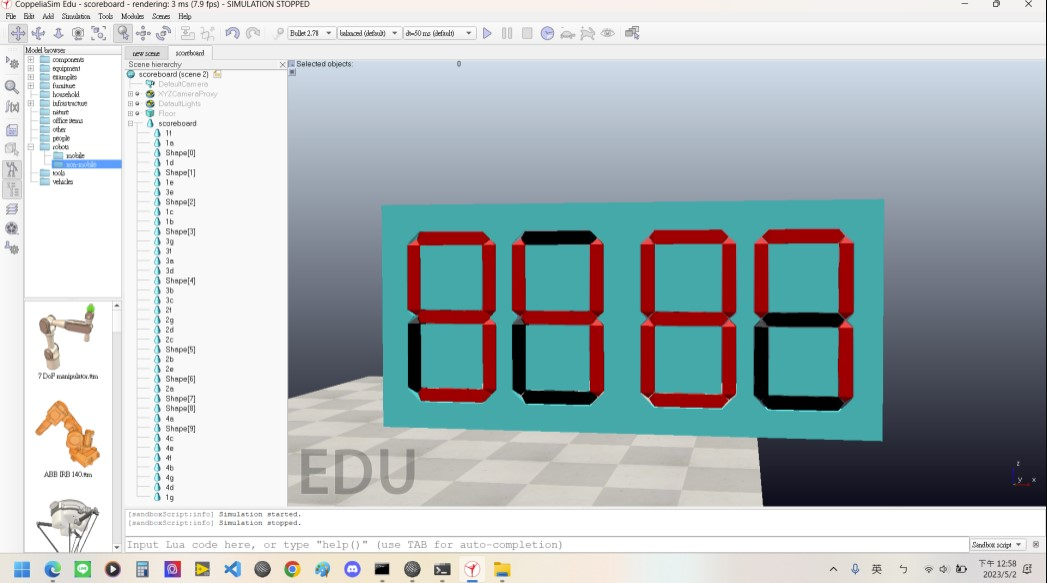
\includegraphics[width=12cm]{9487}
\caption{\Large 變色顯示得分}\label{變色顯示得分}
\end{center}
\end{figure}\\ 
第四版記分板建立,因前面對老師的要求理解錯誤,我們做成隨得分改變顏色的記分板設計,因此做了這版來滿足老師所要求的機械式設計。如(圖.\ref{第四版記分板背面})紅色圓形部分為固定銷,白色圓形部分是可向前推動的銷,可實現將桿件向前推送達成數字顯示的效果。\\
\begin{figure}[hbt!]
\begin{center}
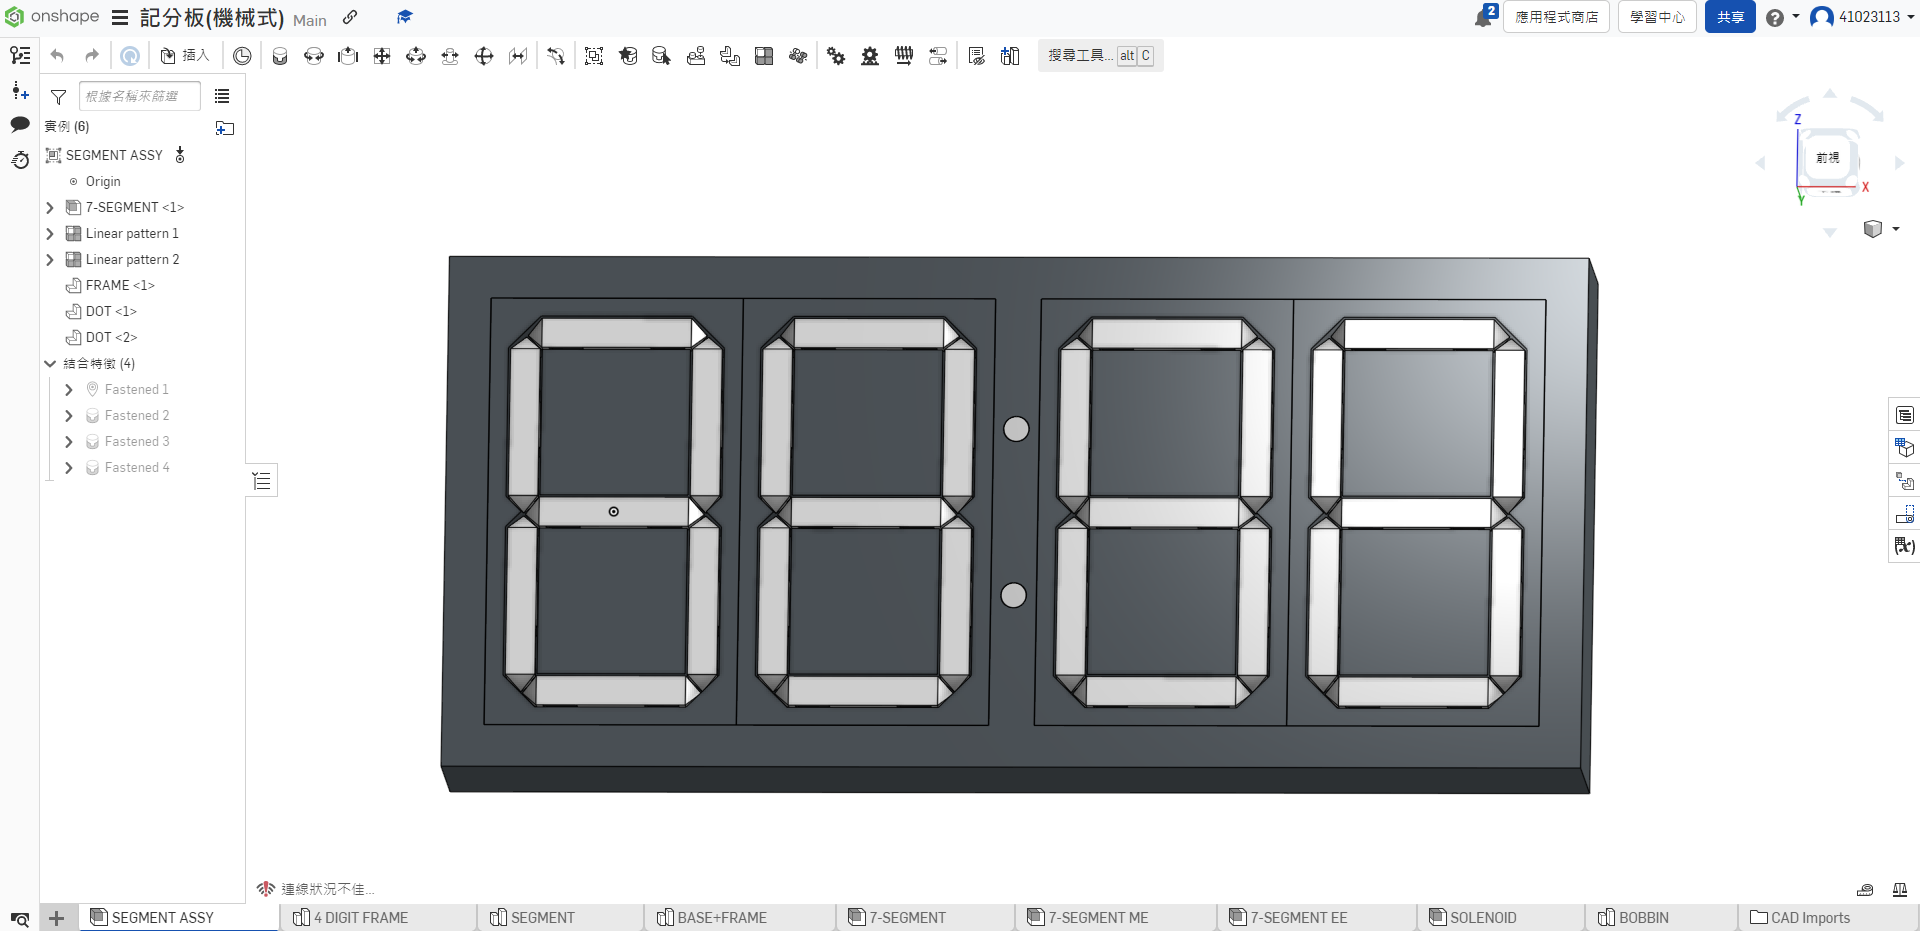
\includegraphics[width=12cm]{記分板1}
\caption{\Large 第四版記分板}\label{第四版記分板}
\end{center}
\end{figure}
\begin{figure}[hbt!]
\begin{center}
\newpage
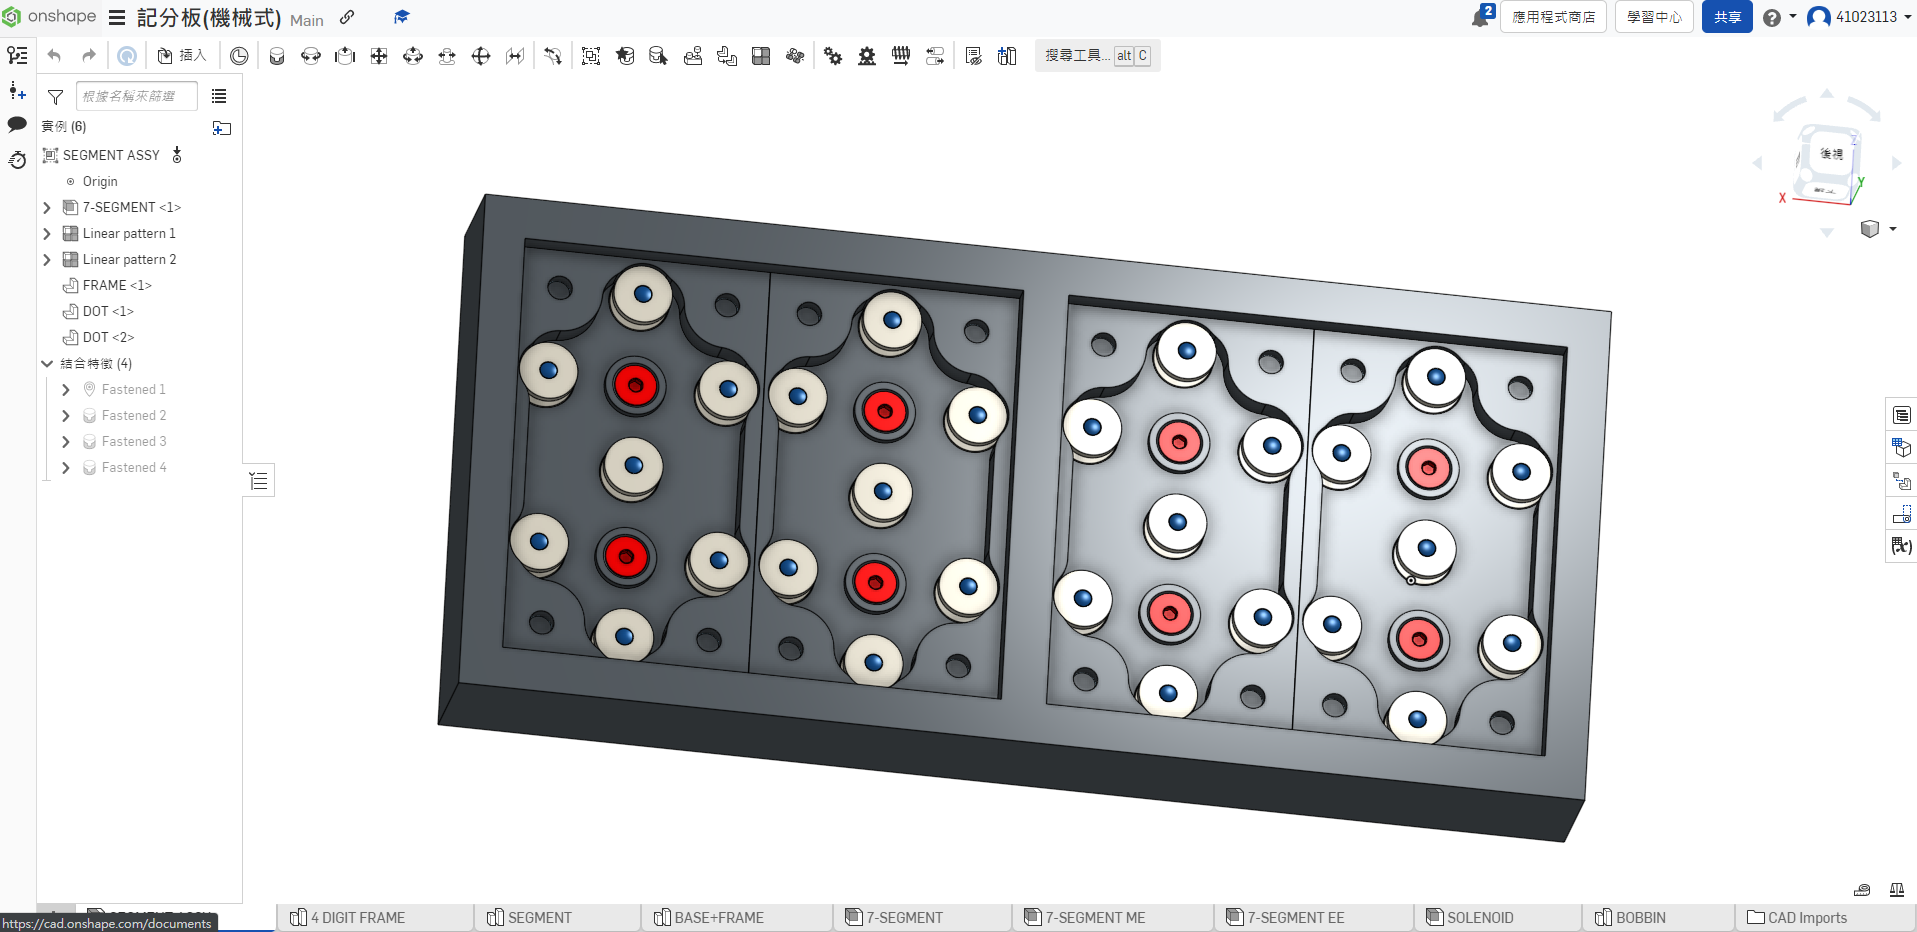
\includegraphics[width=12cm]{記分板2}
\caption{\Large 第四版記分板背面}\label{第四版記分板背面}
\end{center}
\end{figure}
\\
\\
\\
第五版記分板建立,第四版在經過組內討論後,發現顯示效果不太容易判讀,因此建立第五版記分板如(圖.\ref{第五版記分板}),原理大致上與第四版相同,皆是使用joint推動顯示數字如(圖.\ref{第五版記分板原理})。
\begin{figure}[hbt!]
\begin{center}
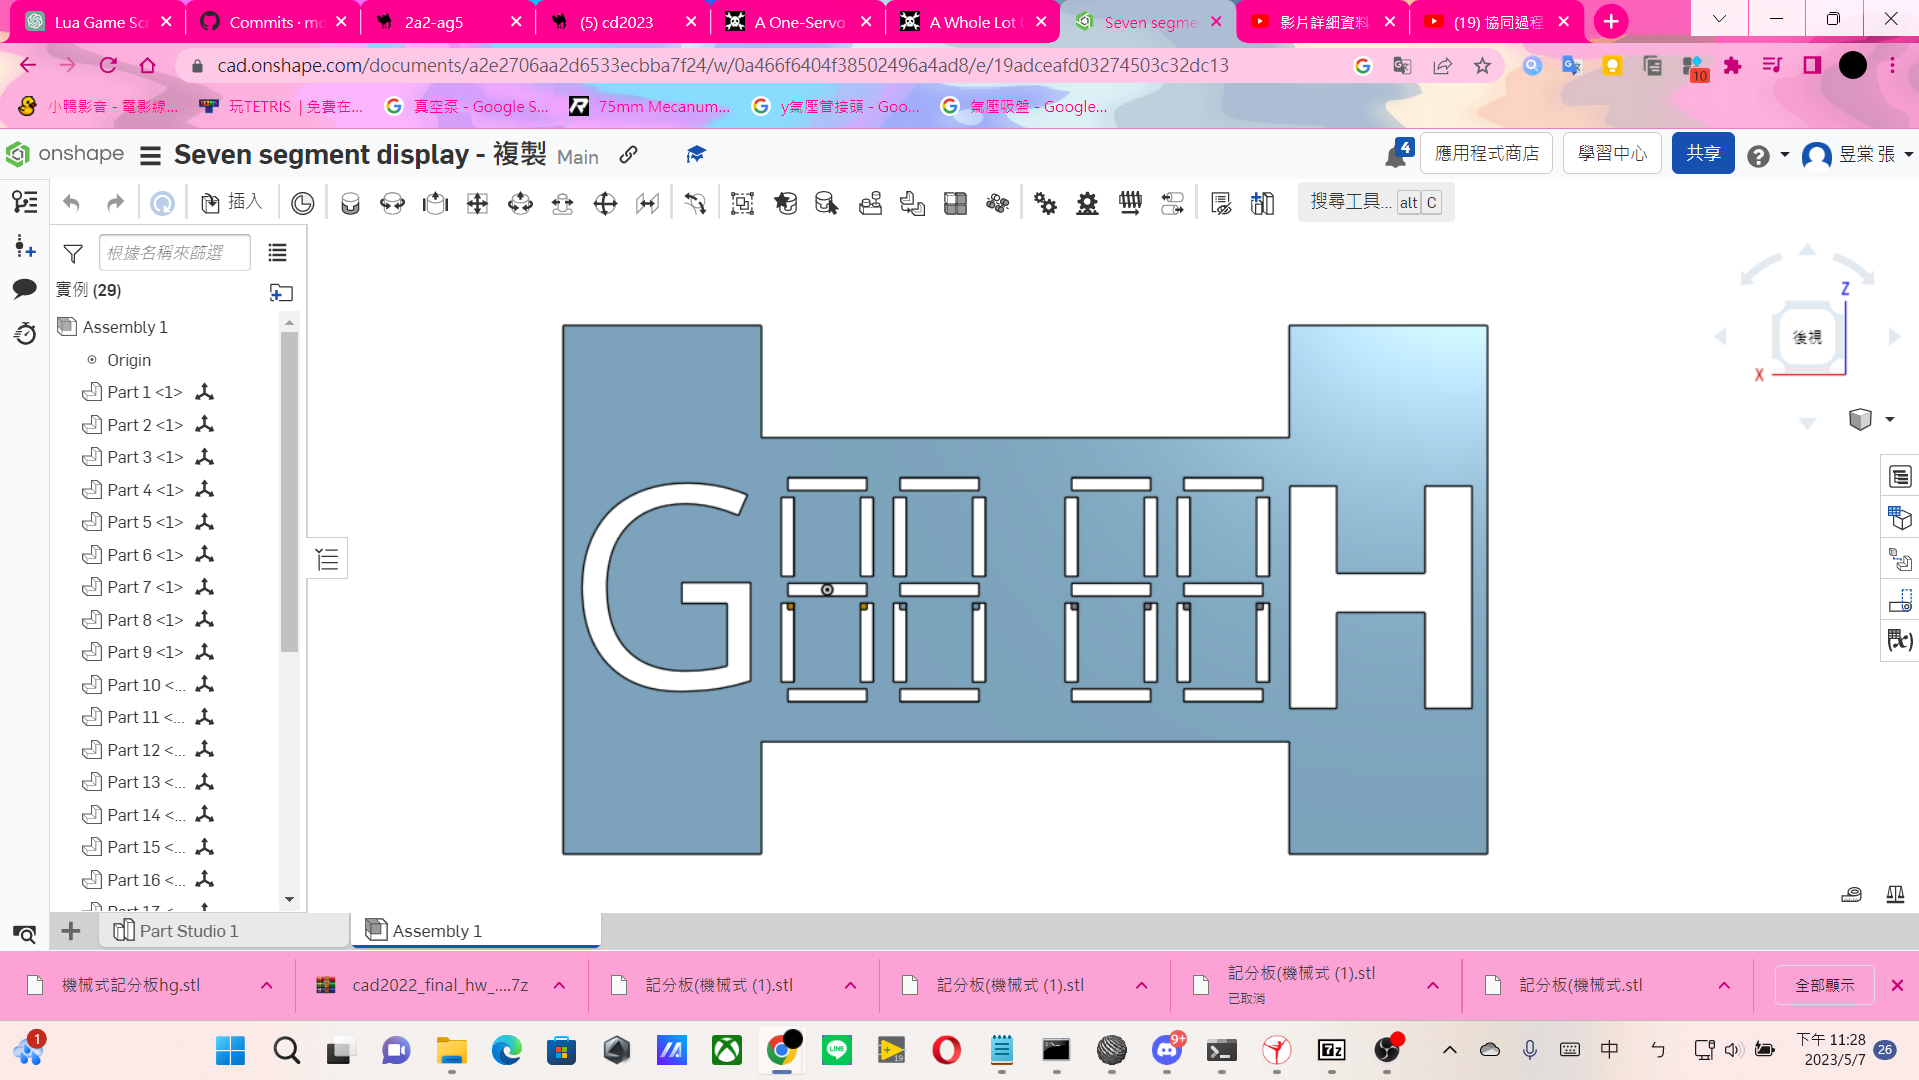
\includegraphics[width=9cm]{機械計分版圖片}
\caption{\Large 第五版記分板}\label{第五版記分板}
\end{center}
\end{figure}
\begin{figure}[hbt!]
\begin{center}
\newpage
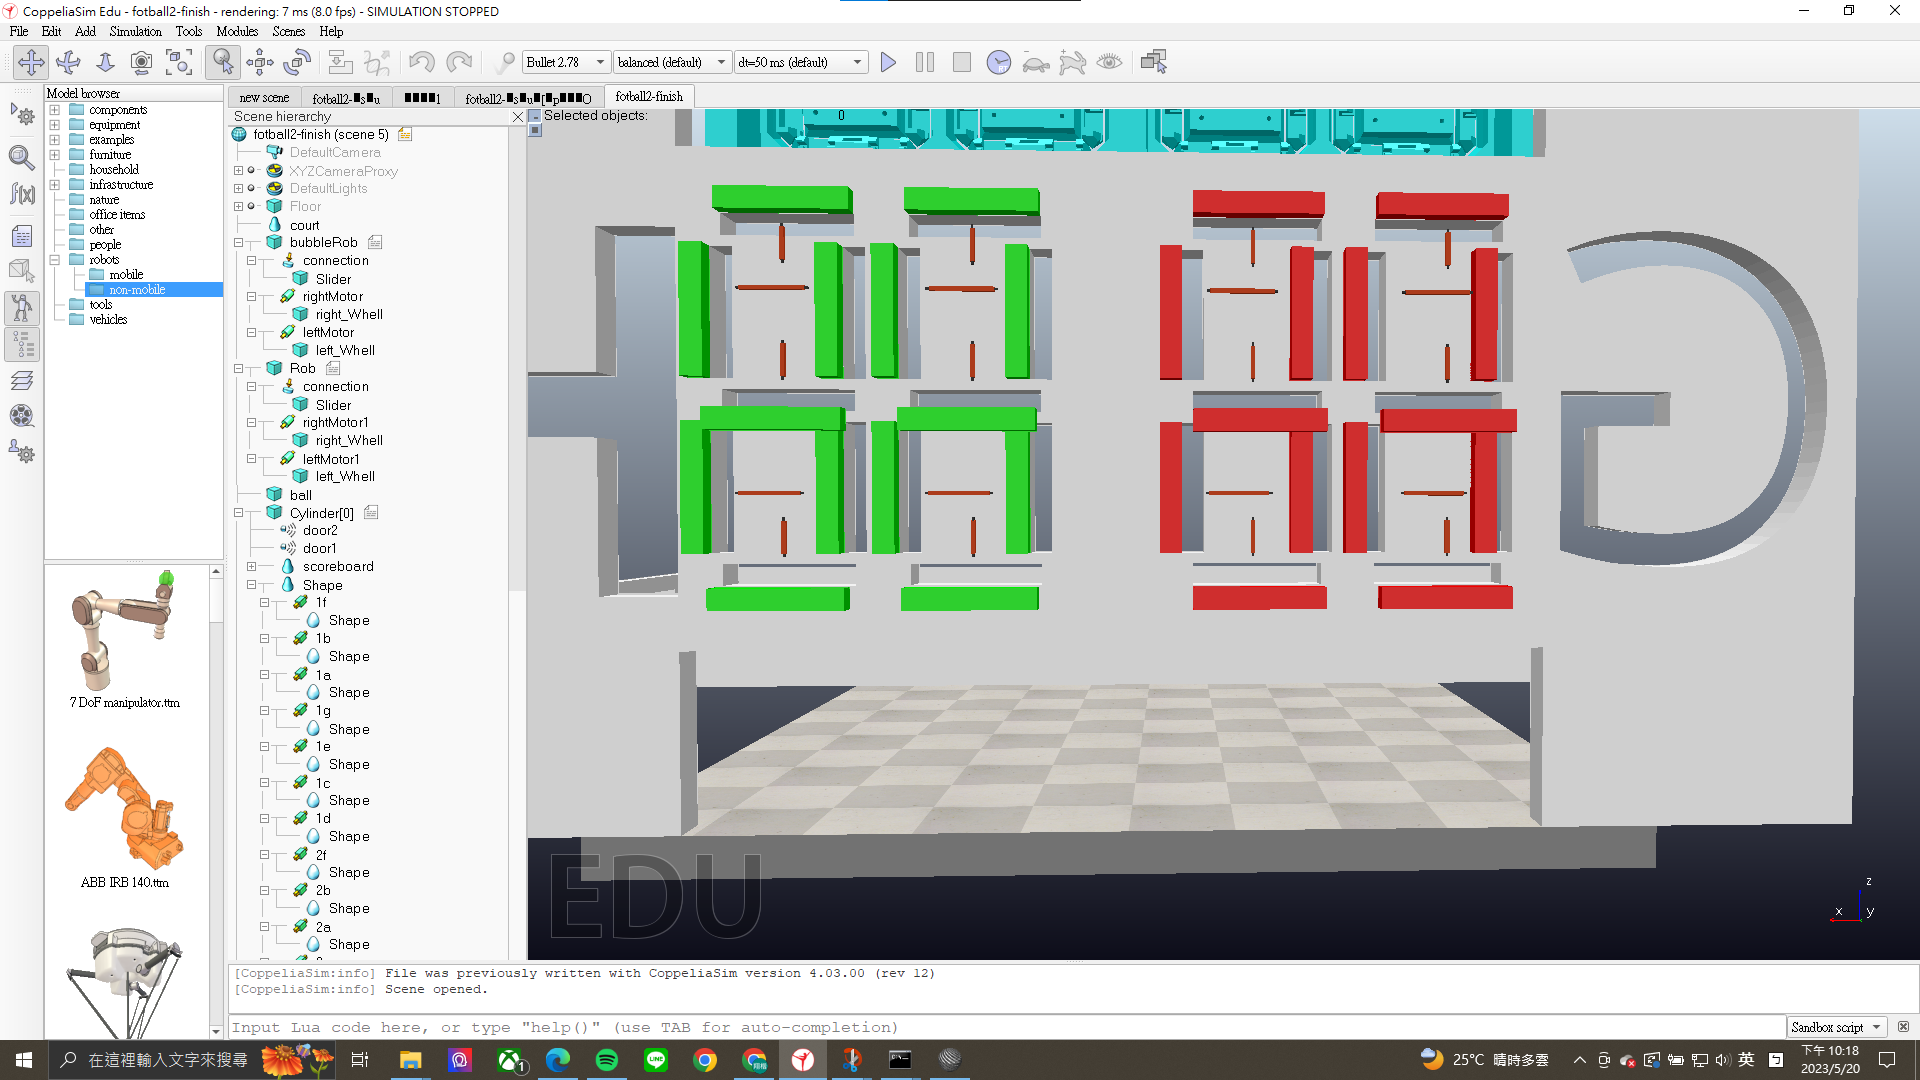
\includegraphics[width=9cm]{5b}
\caption{\Large 第五版記分板原理}\label{第五版記分板原理}
\end{center}
\end{figure}